%%% Econ712: Macroeconomics I
%%% Fall 2020
%%% Danny Edgel
%%%
% Due on Canvas Wednesday September 10, 11:59pm Central Time
%%%

%%%
%							PREAMBLE
%%%

\documentclass{article}

%%% declare packages
\usepackage{amsmath}
\usepackage{amssymb}
\usepackage{array}
\usepackage{bm}
\usepackage{changepage}
\usepackage{centernot}
\usepackage{graphicx}
\usepackage{fancyhdr}
	\fancyhf{} % sets both header and footer to nothing
	\renewcommand{\headrulewidth}{0pt}
    \rfoot{Edgel, \thepage}
    \pagestyle{fancy}
	
%%% define shortcuts for set notation
\newcommand{\N}{\mathbb{N}}
\newcommand{\Z}{\mathbb{Z}}
\newcommand{\R}{\mathbb{R}}
\newcommand{\Q}{\mathbb{Q}}
\newcommand{\lmt}{\underset{x\rightarrow\infty}{\text{lim }}}
\newcommand{\neglmt}{\underset{x\rightarrow-\infty}{\text{lim }}}
\newcommand{\zerolmt}{\underset{x\rightarrow 0}{\text{lim }}}
\newcommand{\usmax}{\underset{1\leq k \leq n}{\text{max }}}

%%% define column vector command (from Michael Nattinger)
\newcount\colveccount
\newcommand*\colvec[1]{
        \global\colveccount#1
        \begin{pmatrix}
        \colvecnext
}
\def\colvecnext#1{
        #1
        \global\advance\colveccount-1
        \ifnum\colveccount>0
                \\
                \expandafter\colvecnext
        \else
                \end{pmatrix}
        \fi
}

%%% define function for drawing matrix augmentation lines
\newcommand\aug{\fboxsep=-\fboxrule\!\!\!\fbox{\strut}\!\!\!}

\makeatletter
\let\amsmath@bigm\bigm

\renewcommand{\bigm}[1]{%
  \ifcsname fenced@\string#1\endcsname
    \expandafter\@firstoftwo
  \else
    \expandafter\@secondoftwo
  \fi
  {\expandafter\amsmath@bigm\csname fenced@\string#1\endcsname}%
  {\amsmath@bigm#1}%
}


%________________________________________________________________%

\begin{document}

\title{	Problem Set \#1 }
\author{ 	Danny Edgel 					\\ 
			Econ 712: Macroeconomics I		\\
			Fall 2020						\\
		}
\maketitle\thispagestyle{empty}

%%%________________________________________________________________%%%

\textit{Collaborated with Sarah Bass, Emily Case, Michael Nattinger, and Alex Von Hafften}
\medskip \\
The price of a share of some stock at time $t$ with perfect forsight is given as:
\[
	p_t=\frac{d+p_{t+1}}{1+r}
\]


%%%________________________________________________________________%%%

\section*{Question 1}
\textbf{Solve for the steady state stock price} $\mathbf{p^*=p_t=p_{t+1}}$
\medskip \\
We can easily solve for $p^*$ by simply substituting $p^*$ for $p_t$ and $p_{t+1}$ in the share price formula and solving for $p^*$:
\begin{align*}
	p^* 		&= \frac{d + p^*}{1+r} \\
	(1+r)p^* 	&= d + p^*				\\
	rp^*		&= d 					\\
	p^*			&= \frac{d}{r}
\end{align*}


%%%________________________________________________________________%%%

\section*{Question 2}
\textbf{Solve for the steady state stock price} $\mathbf{p^*=p_t=p_{t+1}}$
\medskip \\
Given $p_t$ as a function of $p_{t+1}$, we can derive:
\[ 
	p_t = f(p_{t-1}) = (1+r)p_{t-1} - d 
\]
The general, closed-form solution will take the form:
\[
	p_t=c a^t + M = p_t^c + p_t^p
\]
Where $p_t^c=c a^t$ is a complementary solution, $p_t^p$ is a particular solution, and $a=1+r$. Since we know that $p_{t+1}=f(p^*)=p^*$, we can use $p^*$ as a particular solution. Then, since $p_0$ is given, we can use $p_0^g=p_0$ as a boundary solution to solve for $c$:
\begin{align*}
	p_0 &= c a^0 + p^* \\
	c   &= p_0 - p^*
\end{align*}
\smallskip \\
Thus, we arrive at the closed-form solution: $p_t=(p_0-p^*)(1+r)^t+p^*$. Since $r>0$, $1+r>1$. Therefore, $|p_t|$ diverges to infinity unless its initial value is equal to its steady state:
\[
	\underset{t\rightarrow\infty}{\text{lim }p_t} = \begin{cases}	\infty, & p_0 > p^* \\
																	p^*, 	& p_0 = p^* \\
																	-\infty,& p_0 < p^*
													\end{cases}
\]
Each of these outcomes is displayed in the plot below, which plots $p_t$ against $p_{t+1}$ for $t=\{1,...,300\}$. The black line (dot) shows the relationship when $p_0=p^*$, the blue line plots it when $p_0=p^*+1$, and the red line plots it when $p_0=p^*-1$
\begin{center}
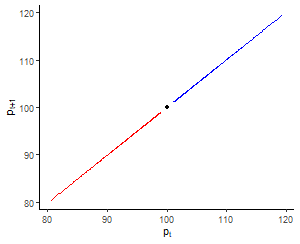
\includegraphics[scale=1]{problem2_phaseplot.png}
\end{center}
The same series are plotted below, using the same color scheme for each series, with $t$ plotted on the $x$-axis and $p_t$ plotted on the $y$-axis.
\begin{center}
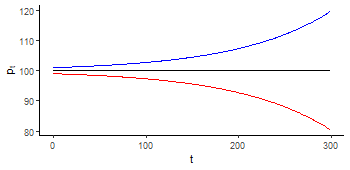
\includegraphics[scale=1]{problem2_timeplot.png}
\end{center}



%%%________________________________________________________________%%%

\section*{Question 3}
\textbf{Modify the code provided to plot the price dynamics over 100 periods with three different initial prices which are respectively blow, at, and above the steady state price level}
\medskip \\
The requested chart is below, which was generated using R. I know Matlab enough to translate between the two, but I prefer to use R. The red line uses $p_0=110$, and the blue line uses $p_0=90$.
\begin{center}
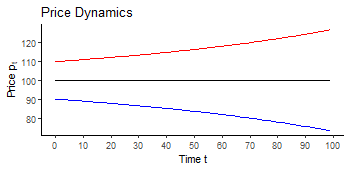
\includegraphics[scale=1]{problem3_timeplot.png}
\end{center}


%%%________________________________________________________________%%%

\section*{Question 4}
\textbf{Suppose the Federal Reserve announces at} $\mathbf{t = 20}$ \textbf{to raise the federal funds rate from} $\mathbf{1\% \text{ to } 2\% \text{ at } t = 50}$ \textbf{and remain at the new level forever. Using (1) with} $\mathbf{d = 1}$\textbf{; how does the price respond to the policy announcement and the interest rate change over time? Plot the price dynamics from} $\mathbf{t = 0}$ \textbf{to} $\mathbf{t = 99}$\textbf{.}
\medskip \\
Beginning at time $t=20$, the price at time $t$ accounts for $p_{50}=50$. Since $p_t=\frac{d+p_{t+1}}{1+r}$, the knowledge that $p_{50}=50$ at $t=20$ leads investors to price the stock lower in each period from $t=20$ to $t=49$ even though $r$ has not yet changed. This takes the form of a steep, one-time drop in period $t=20$ following the news, then a slow convergence to $p_{50}$ over the next 30 time periods, as the plot below shows.
\begin{center}
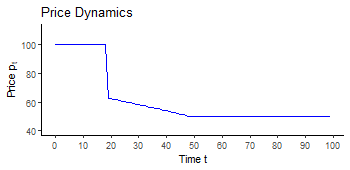
\includegraphics[scale=1]{problem4_timeplot.png}
\end{center}



%%%________________________________________________________________%%%


\end{document}












